\section{Racionální lomená funkce}
\begin{definition}
    Nechť $k \in \mathbb R, k \ne 0.$ Pak funkcí $y=\frac{k}{x}$
    nazýváme \textbf{nepřímou úměrností} s~koeficientem nepřímé úměrnosti $k$.
\end{definition}

\begin{definition}
    Nechť $a,b,c,d \in \mathbb R, c \ne 0, ad-bc \ne 0.$ Pak funkci
    $f:y=\frac{ax+b}{cx+d}$ nazýváme \textbf{lineární lomenou
    funkcí}.
\end{definition}

\begin{figure}[ht!]
  \centering
  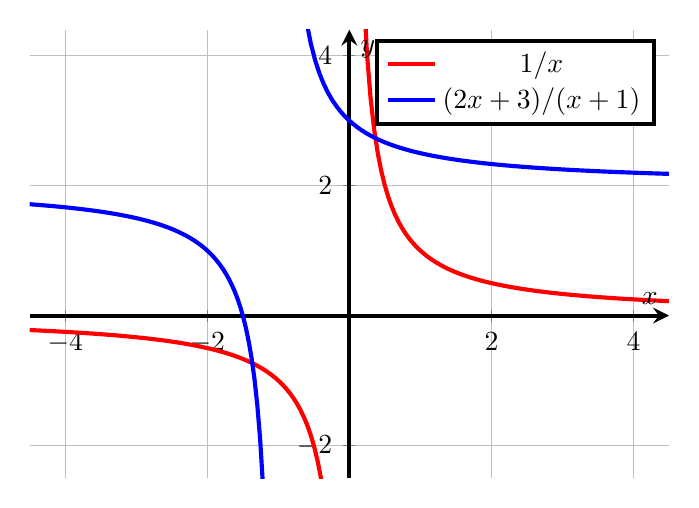
\begin{tikzpicture}
    \begin{axis}[
        axis lines = middle,
        xlabel = \(x\),
        ylabel = {\(y\)},
        line width=1.5pt,
        width=.8\textwidth,
        height=.6\textwidth,
        ymin=-2.5,
        ymax=4.4,
        xmin=-4.5,
        xmax=4.5,
        grid
    ]
    %Below the red parabola is defined
    \addplot [
        domain=-5:-0.1,
        samples=100,
        color=red
    ]
    {1/x};
    \addplot [
        domain=-5:-1.1,
        samples=100,
        color=blue
        ]
        {(2*x+3)/(x+1)};
    \addplot [
        domain=0.1:5,
        samples=100,
        color=red
    ]
    {1/x};
    \addlegendentry{\(1/x\)}


    \addlegendentry{\((2x+3)/(x+1)\)}
    \addplot [
        domain=-0.9:5,
        samples=100,
        color=blue
        ]
        {(2*x + 3) / (x+1)};


    \end{axis}
    \end{tikzpicture}
\label{reseniobr}
  \caption{Grafy různých lineárně lomených funkcí}
\end{figure}

\begin{priklad}
Nakreslete graf funkce $f: y=\frac{2x+3}{x+1}.$
\end{priklad}

\begin{reseni}
Vydělením získáme přehled o posunech počátku:
\begin{equation*}
	(2x+3):(x+1)=2+\frac{1}{x+1}.
\end{equation*}
Hyperbola je tedy posunutá o dva nahoru a o jedna doleva. Přesvědčit se můžeme v obrázku \ref{reseniobr}.
\end{reseni}

\begin{pozn}
  Pro lineární lomenou funkci platí
  \begin{itemize}
      \item $D(f)=\mathbb R \smallsetminus \left \{ -\frac{d}{c} \right \},$
    	\item $H(f)=\mathbb R \smallsetminus \left \{ \frac{a}{c} \right \},$
     	\item grafem je rovnoosá hyperbola s asymptotami
      $x=-\frac{d}{c}, y=\frac{a}{c}.$
  \end{itemize}
\end{pozn}

\begin{veta}
    Lineární lomená funkce:
    \begin{enumerate}[$i.$]
        \item není ani sudá, ani lichá;
       	\item $bc-ad > 0 \implies$ klesající v
        $\left ( -\infty, -\frac{d}{c} \right ),
        \left ( -\frac{d}{c}, \infty \right ) $ \\
        $bc-ad < 0 \implies$ rostoucí v
        $\left ( -\infty, -\frac{d}{c} \right ),
        \left ( -\frac{d}{c}, \infty \right ) $;
       	\item není omezená ani shora, ani zdola;
       	\item nemá extrémy;
       	\item není periodická;
       	\item je prostá.
    \end{enumerate}
\end{veta}

\begin{definition}
    Nechť $P(x), Q(x) \mathbb R[x]$ jsou polynomy, $Q(x) \ne O(x).$
    Pak funkci $F:y=\frac{P(x)}{Q(x)}$ nazýváme \textbf{racionální
    lomenou funkcí}.
\end{definition}

\begin{definition}
    Racionální lomená funkce $f: y=\frac{P(x)}{Q(x)}, Q(x) \ne O(x)$
    se nazývá
    \begin{enumerate}[$i.$]
        \item \textbf{ryze lomená} racionální funkce
        $\iff \text{st}\left (P(x) \right ) <
        \text{st}\left (Q(x) \right )$;
       	\item \textbf{neryze lomená} racionální funkce
        $\iff \text{st}\left (P(x) \right ) \geq
        \text{st}\left (Q(x) \right )$.
    \end{enumerate}
\end{definition}

\begin{priklad}
  Určete, pro která $x \in \mathbb R$ platí
  $$P(x) = \frac{(x-1)^2(x+5)^3x^4(x^2-5x+6)(x^2+1)(x-5)^5}{(x-3)^3(x^2+7)} \geq 0.$$
\end{priklad}

\begin{reseni}
  Rozložíme čitatele i jmenovatele v reálném oboru. Znaménko se obecně mění v~kořenech čitatele nebo kořenech jmenovatele. Členy se záporným diskriminantem nemají reálný kořen,
  neuvažujeme je tedy. V~sudých mocninách se nemění znaménko. Zároveň musíme vyloučit samotné kořeny jmenovatele, protože je v nich výraz nedefinován. Toto vše vyneseme na číselnou osu.
\end{reseni}

\begin{veta}[Rozklad na parciální zlomky]
    Nechť $f: y=\frac{P(x)}{Q(x)}, Q(x) \ne O(x)$ je ryze lomená
    racionální funkce, kde polynomy $P(x)$ a $Q(x)$ nemají společné
    kořeny. Nechť
    \begin{align*}
        Q(x) = & \, a_n(x-c_1)^{k_1}(x-c_2)^{k_2} \dots
        (x-c_l)^{k_l} \\
        \cdot & \, (x^2+p_1x + q_1)^{r_1}(x^2+p_2x+q_2)
        ^{r_2} \dots (x^2+p_sx+q_s)^{r_s}
    \end{align*}
    je rozklad polynomu $Q(x)$ v reálném oboru. Pak existují čísla
    \begin{center}
        \begin{tabular}{l l l l}
            $C_{11}$, & $C_{12}$, & $\dots$, & $C_{1k_1}$, \\
            $C_{21}$, & $C_{22}$, & $\dots$, & $C_{2k_2}$, \\
            \,        & \,        & $\dots$  & \,          \\
            $C_{l1}$, & $C_{l2}$, & $\dots$, & $C_{lk_l}$; \\
            $P_{11}$, & $P_{12}$, & $\dots$, & $P_{1r_1}$, \\
            $P_{21}$, & $P_{22}$, & $\dots$, & $P_{2r_2}$, \\
            \,        & \,        & $\dots$  & \,          \\
            $P_{s1}$, & $P_{s2}$, & $\dots$, & $P_{sr_s}$; \\
            $Q_{11}$, & $Q_{12}$, & $\dots$, & $Q_{1r_1}$, \\
            $Q_{21}$, & $Q_{22}$, & $\dots$, & $Q_{2r_2}$, \\
            \,        & \,        & $\dots$  & \,          \\
            $Q_{s1}$, & $Q_{s2}$, & $\dots$, & $Q_{sr_s}$
        \end{tabular}
    \end{center}
    tak, že $\forall x \in \mathbb R$ platí
    \begin{align*}
        y = & \left [
              \frac{C_{11}}{x-c_1} + \frac{C_{12}}{(x-c_1)^2} +
              \dots + \frac{C_{1k_1}}{(x-c_1)^{k_1}} \right . \\
          & + \frac{C_{21}}{x-c_2} + \frac{C_{22}}{(x-c_2)^2} +
              \dots + \frac{C_{2k_2}}{(x-c_1)^{k_2}} \\
          & + \dots \\
          & + \frac{C_{l1}}{x-c_l} + \frac{C_{l2}}{(x-c_l)^2} +
              \dots + \frac{C_{lk_l}}{(x-c_l)^{k_l}} \\
          & + \frac{P_{11}x + Q_{11}}{x^2 + p_1x + q_1}
              + \frac{P_{12}x + Q_{12}}{(x^2 + p_1x + q_1)^2} + \dots
              + \frac{P_{1r_1}x + Q_{1r_1}}{(x^2 + p_1x + q_1)^{r_1}} \\
          & + \frac{P_{21}x + Q_{21}}{x^2 + p_2x + q_2}
              + \frac{P_{22}x + Q_{22}}{(x^2 + p_2x + q_2)^2} + \dots
              + \frac{P_{2r_2}x + Q_{2r_2}}{(x^2 + p_2x + q_2)^{r_2}} \\
          & + \dots \\
          & + \left . \frac{P_{s1}x + Q_{s1}}{x^2 + p_sx + q_s}
              + \frac{P_{s2}x + Q_{s2}}{(x^2 + p_sx + q_s)^2} + \dots
              + \frac{P_{sr_s}x + Q_{sr_s}}{(x^2 + p_sx + q_s)^{r_s}} \right ]
              \cdot \frac{1}{a_n}
    \end{align*}
\end{veta}

\begin{priklad}
Rozložte na parciální zlomky: $y=\frac{x-4}{x^2-5x+6}.$
\end{priklad}

\begin{reseni}
Platí
$$\frac{x-4}{x^2-5x+6}=\frac{A}{x-2}+\frac{B}{x-3}.$$
Metodou porovnání koeficientů tedy řešíme rovnici $x-4=A(x-3)+B(x-2)$.
\end{reseni}
